\documentclass{article}
\usepackage{graphicx} % Required for inserting images

\title{Final Report of Capstone project}
\author{
  Debasish Das\\
  \texttt{d.das@student.fdu.edu}
  \and
  Sai Nithish Reddy Madireddy\\
  \texttt{s.madireddy@student.fdu.edu}
  \and
  Sanad Mukadam\\
  \texttt{s.mukadam@student.fdu.edu}
}
\date{21 July 2023}

\bibliographystyle{plain}
\usepackage[hyphens,spaces]{url}

\begin{document}

\maketitle

\section{Introduction}
The project devise an web application named 'nav-route' where a user can find a set of optimized routes to visit single or multiple destinations from the source based on shortest distance with priority, and safety concerns such as left turns, right turns, total turns etc. Travellers, delivery persons, business-people and others need to go to different places or locations. Their preferences differ based on distance, priority, safety, cost and other criteria. If the number of destinations is N, there are N! possible routes, and it is hard to find the suitable route based on the user's preference. The web application, 'nav-route', provides a user-friendly intuitive interface to solve this problem. The intended user will be able to find his/her preferred routes by distance in ascending order with option for putting priority weight on destination, and sorting them with number of turns. Then s/he can see the details with map in this application. Initially, it shows top five routes instead of showing N! routes. If the user is interested to check more routes, s/he can click the button for showing more routes. It makes the application user-friendly and lightweight. Because the direction information of each route requires an API call with a compressed response size of 10 kilobytes. However, the user will need to sign in to the web application to use it.

\section{Related work}
Route4Me provides the shortest route for its customers to go to multiple locations avoiding left turn for fuel efficiency and safety\cite{r1}. Waze provide routing information regarding live update, construction and other criteria\cite{r2}. Google map allows adding multiple destinations or stops\cite{r3}. Here, we could not find the shortest routes for multiple destinations. On the other hand, the project focuses on providing service to generate optimized route for multiple destinations based on user's preferences like setting priority or weight on safety, distance or others. 

\section{Methodologies}

Kan-ban based on Trail-and-Error methodology has been used to solve the problem for this project. The tasks were broken down and distributed among the team members in the Kan-ban board of trello site. A product backlog was maintained for the tasks with less priority. This methodology with Kan-ban was suitable for a small team working on a problem solving project that is going to end within a short period. Here, planning and design often changed for the effective and time-saving solution of the web application.

\subsection{Front-end}
OpenStreetMap and Google Maps Platform API were explored to extract information for routing. The team could not make enough progress with OpenstreetMap to integrate it to the main application in due time. Meanwhile, the team could explore Google Maps Platform API enough to use it in the application. It has lots of examples, demo and documentation available. At first, only the Direction map API with way-points was planned to use. However, it could have been too expensive in terms of memory, processing and number of API calls. If the number of destinations had been 7, there could have been 7! or 5040 API calls with 10KB http response size for each call. The Google Distance Matrix API came up with a solution for this problem. After calling this API,  Heap's Algorithm was used to find the all the possible routes with distance and time. The callback output from Heap's algorithm were modified to prioritize destinations and sort the routes the according to the user preferences. For single destination, the application is able to generate at most three alternative routes. For number of N destinations, it is possible to generate at most N! routes. Then, the google map Direction API with way-point is called for top five routes that can be rendered in the map with google map Render API. By user preferences, more routes can be fetched, and shown on map. These features are parts of front-end Single Page Application of ES6 Module.
\\
\\
Google oAuth and some UI design features were also developed for front-end application. However, those could not be integrated due to time constraint. These features along with OpenstreetMap API are available in the 'Playground' folder of GitHub repository of the project. Some of the other unfinished progresses are also available in the different branch. 

\subsection{Back-end}
A back-end Web-API was also developed for user authentication, storing user information, and to accommodate business information for the front-end application. This Web-API was developed using Ruby on Rails web framework with PostgreSQL database. We switched to Ruby on Rails from .NET core, because it offers powerful scaffolding for Models (that maps as database entity) and Controllers. The cookie based authentication of Ruby on Rails made the integration to front-end web application fast. It also provided packages for user authentication encrypted password and session. Although .NET core provides all these features, being more familiar with cookie based authentication of rails API made the change of decision.The Software Architecture of web application developed for the project is illustrated in Figure 1.

\begin{figure}
  \centering
  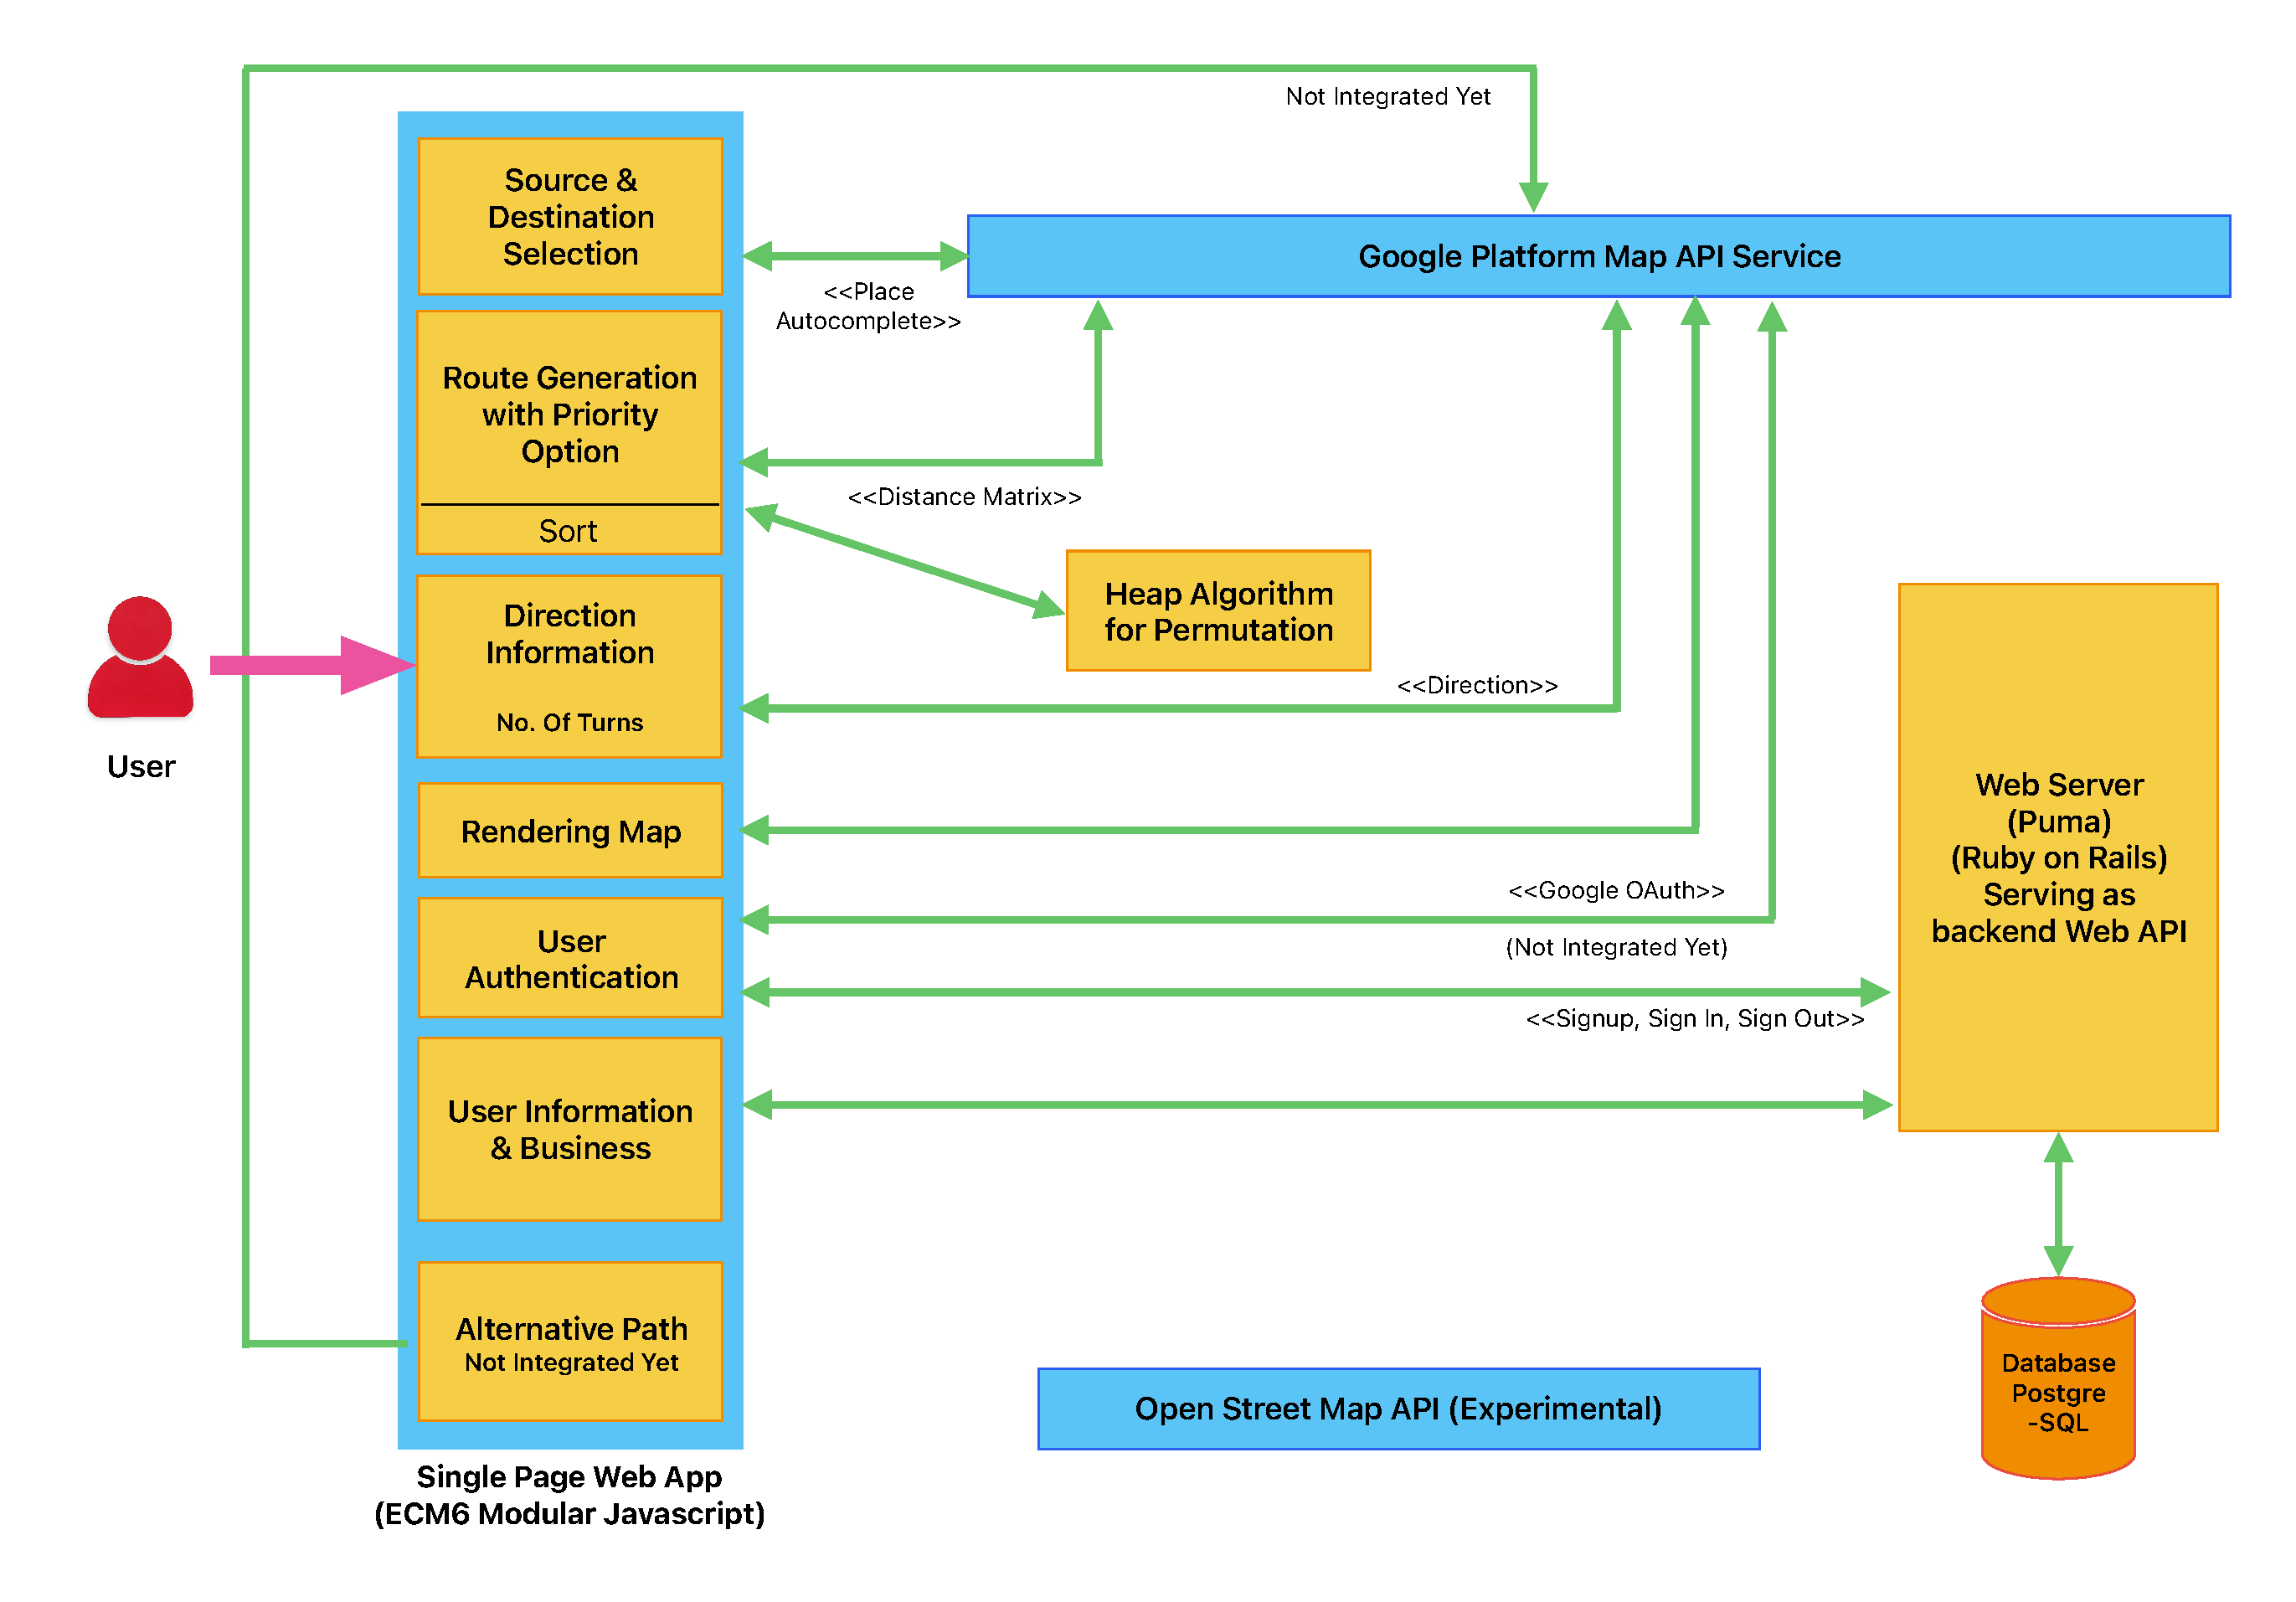
\includegraphics[width=1\textwidth]{Architecture_v2.pdf}
  \caption{Architecture of Nav-Route}
  \label{fig:example}
\end{figure}

\subsection{GitHub}
The link to the GitHub repository of the project is https://github.com/debasish-das/nav-route. The stable version of the application is in main branch. The README.md file of the repository provides technical detail on how to run and setup the project as following:
\\
\\
\begin{verbatim}
## Frontend Web App
### ES6 Module Application
Path: ./WebApp

Resources: https://developers.google.com/maps/documentation, https://developer.mozilla.org/en-US/docs/Web/JavaScript/Guide/Modules

App initiating JS: `WebApp/scripts/main.js`

External JS Libraries:
* https://maps.googleapis.com/maps/api/js
* bootstrap.js (Version: 5)
* polyfill.min.js

External CSS Libraries:
* bootstrap.min.css (Version: 5)

#### Steps to Run:
* Add google map api `YOUR_APP_KEY` in the `index.html`
```
<script 
        src="https://maps.googleapis.com/maps/api/js?key=YOUR_APP_KEY&libraries=places"
        ></script>
```
* Live server extenstion from VS code can be used to run the frontend in development environment. Then clicking the `Go Live` button at bottom right.
* Or, if we have NodeJs, we can install `http-server` with npm. Then, run the command `http-server ./WebApp -p 8088`
* Or, we can ran run it any sever that has port 8088 or 5500

## Backend WebAPI
### Rails API 
Path: ./WebApp

Recources: https://guides.rubyonrails.org/, https://guides.rubyonrails.org/api_app.html

#### Steps to run:
* Install postgresql
* Install ruby on rails
* Go to the `WebApi` directory and run the following commands:
```
bundle
rails db:create
rails db:migrate
rails server
```
\end{verbatim}


\section{Retrospective Observations}
\subsection{What went well}
-Development a lightweight web application that meets the requirement of the Minimum viable product.\\
-Most of the plans to solve the problem worked out. Some required change of plan but it was successful and effective. \\
\subsection{What could be done better}
-The React Framework could make the front-end software development faster and easier. Then it could also be easier to implement the front-end for Mobile platforms.\\
-The code for generating routes and direction with user preference should be at the back-end so that it can be re-used as SAAS, and for other platforms or devices.\\

\section{Challenges}
-Choosing between OpenstreetMap and Google Map Platform API\\
-Accommodating heap algorithm with the response of Distance Matrix API\\
-Limiting the number of Direction API call\\
-Generating the routes based on prioritized destinations\\
-Sorting the routes based on left, right and total number of turns\\
-Integration of the work done by different team members


\section{Team & Individual Accomplishments}
The team has managed to successfully complete the MVP as listed in the proposal. Here are some of the specific milestones that has been achieved listed under each team member responsible for driving them.

\subsection{Debasish Das: Main Application, Architecture, Problem-solving and Documentation}
Debasish Das is responsible for the following:\\
-Developing Single page application of ES6 module\\
-Developing Web API with Ruby on Rails and database PostgreSQL\\
-Generating routes from google distance matrix, heap algorithm, and showing the route information with google direction api according the user preference by priority and number of turns with efficiency and user friendly UI\\
-Cookie based authentication with Rails Web API\\
-Distributing and Integrating work done by other team members in the main application\\
-Documentation in Mark down (README.md) and latex (Introduction, Methodologies, Retrospective Observations and Challenges)

\subsection{Sai Nithish: OpenstreetMap API, Single-Source-Single-Destination Problem, Architecture, Documentation }
OpenStreetMap API:
I worked with the OpenStreetMap API, a project that offers free and editable map data, along with Application Programming Interfaces (APIs) for accessing and utilizing this data in applications. Several APIs are available for accessing OSM data and services. I initially used Leaflet and MapBox API to create a working version of the application. However, due to certain constraints and design choices, eventually we switched from OSM to the Google Maps API.
\\
\\
SingleSource-SingleDestination Problem:
While the DistanceMatrix service is useful for getting multiple route suggestions for more than one destination, it has limited functionality when dealing with a single source and single destination. This led to the need for a service that can fetch multiple routes in the case of Single-Source-Single-Destination scenarios. After exploring documentation and various solutions, I discovered the Direction service, which is also part of the Google Maps API. It accepts the origin, destination, driving mode, and a flag called provide Alternate Routes as part of the request, and in response, it provides geocoded waypoints. This response is then parsed, and the turns are calculated. Based on user preferences for sorting (e.g., total turns, left turns, right turns), multiple routes are displayed along with their estimated time of arrival (ETA) and distance. When the user selects a route and clicks on the "showMap" button, the corresponding route will be displayed on the map.
\\\\
Technologies Used:  \\
●	Web – HTML 5, CSS3, Bootstrap 5, JavaScript, Google-Maps API(Direction Service).\\
●	IDE: Visual Studio Code 1.79 \\
I worked on the JS files for placing a request to Maps API Direction service and then by parsing the response gathered the turns data for individual routes. This data is then sent over to a function which generates the HTML view which has the rendered turns data along with ETA and distance.

\subsection{Sanad Mukadam: UI Design, Architecture, Autocomplete, Authentication, UI Integration, Report}
Address Lookup & Autocomplete using Google Maps API: 
The Address lookup and autocomplete feature is an important aspect of our project. It is important for the user to be able to type in an address and be able to access autocompletion of addresses based on suggestions generated by the API used for lookup. \\
Technologies Used:  \\
●	Web – HTML 5, CSS3, Bootstrap 5, JavaScript \\
●	IDE: Visual Studio Code 1.79 \\
●	Graphic Editor: Adobe Photoshop \\
 
●	Developed web page in HTML using CSS, JavaScript, and Bootstrap to allow user to enter Address and gives type-ahead-search functionality of Google map search field. The autocomplete service can match on full words and substrings, resolving place names, addresses,  \\
●	Embedded Google API to accomplish the task. \\
●	Developed webpage giving user two options  \\
o	to enter address in one text box, \\
o	to enter address in first text box, based on which it will autofill other details like street address, city, state, zip code, country.  \\
●	Uploaded webpage to GitHub repository. \\
 
Architecture Design & Drawing: \\
Architecture design and concept was discussed with the team and was implemented after careful consideration of the elements of our project. 
 
Technologies Used:  \\
●	Drawing tool - Apple Freeform 1.2 for MacOS
UI Design Hand-sketched Concept: \\
The UI is an important part of any application. Several sketches were prepared after consultation with the team and agreed upon drafts were uploaded to the Git repository. At the end, we intend to integrate the application with the front end. The concept drawing of the UI, therefore was a great idea that allowed us to envision how we wanted the app to look and function. Also, it offers a unique way to anticipate the flow of the program and allows us to take steps in making the interface easy to use and maintain.


\begin{figure}
  \centering
  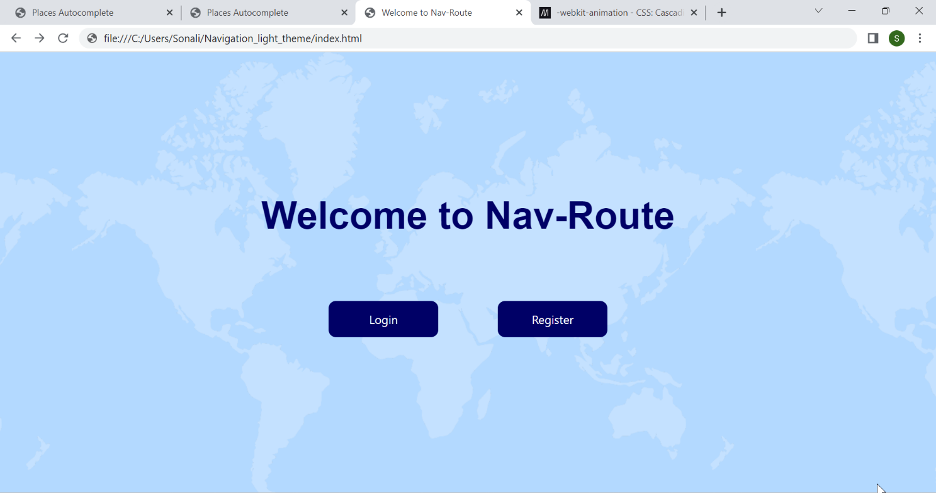
\includegraphics[width=1\textwidth]{NithishFinal/Picture5.png}
  \caption{Animated-background-theme }
  \label{fig:example}
\end{figure}

\begin{figure}
  \centering
  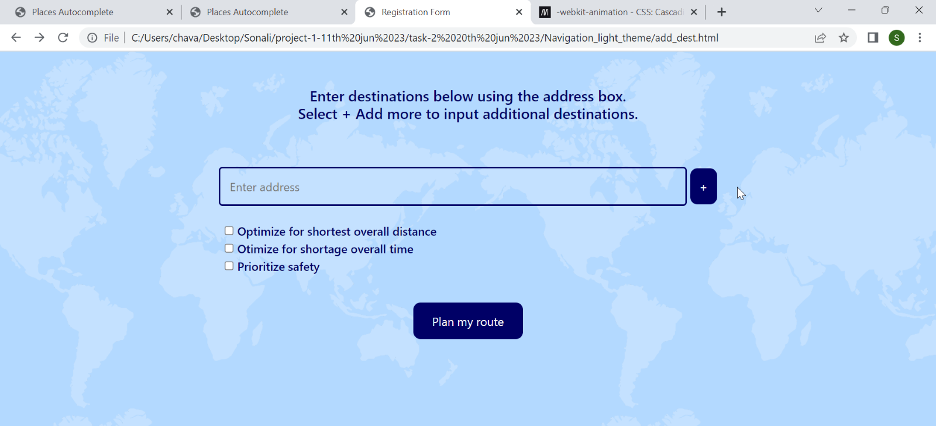
\includegraphics[width=1\textwidth]{NithishFinal/Picture6.png}
  \caption{Animated-background-theme }
  \label{fig:example}
\end{figure}

\begin{figure}
  \centering
  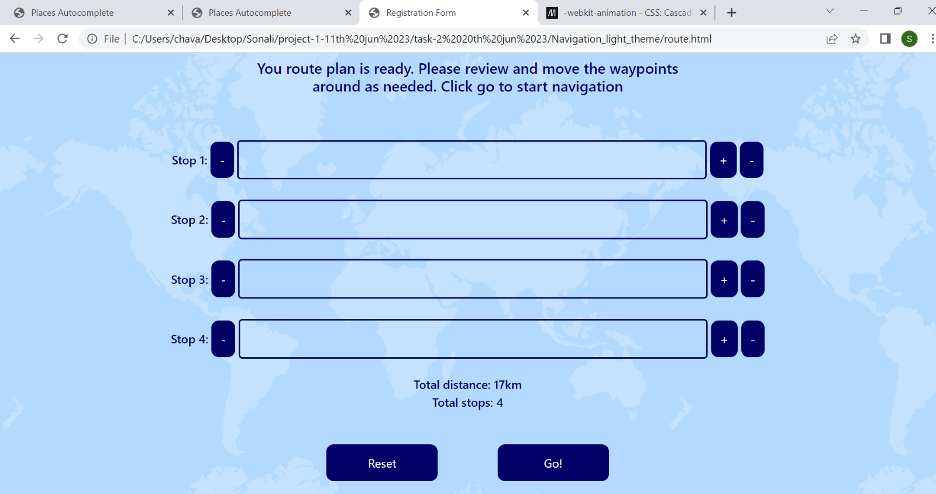
\includegraphics[width=1\textwidth]{NithishFinal/Picture7.png}
  \caption{Animated-background-theme }
  \label{fig:example}
\end{figure}

\begin{figure}
  \centering
  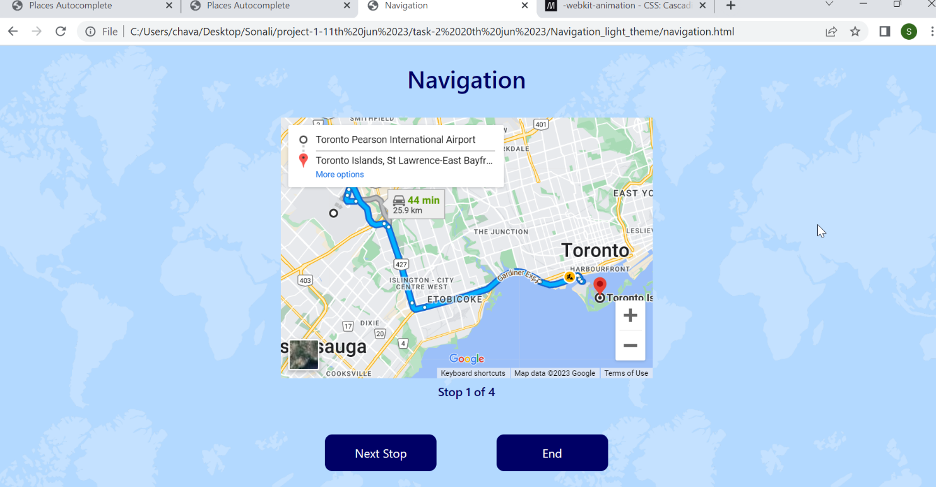
\includegraphics[width=1\textwidth]{NithishFinal/Picture8.png}
  \caption{Animated-background-theme }
  \label{fig:example}
\end{figure}

\begin{figure}
  \centering
  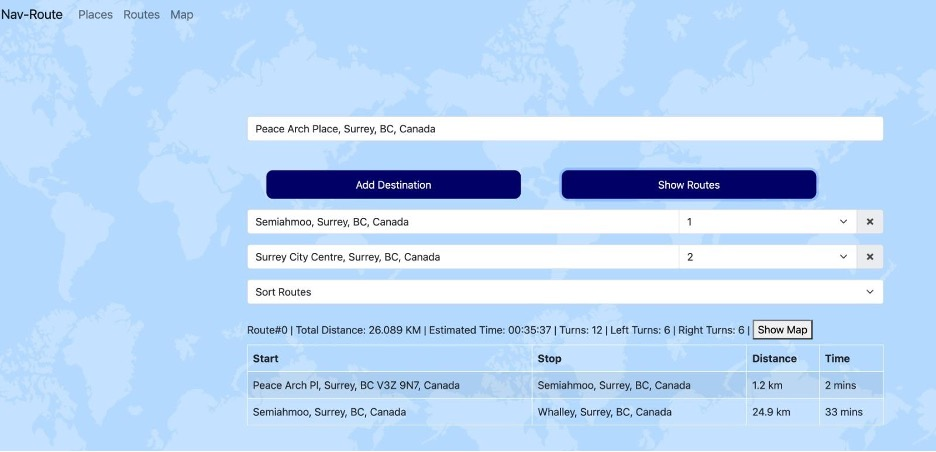
\includegraphics[width=1\textwidth]{NithishFinal/Picture9.jpg}
  \caption{Animated-background-theme }
  \label{fig:example}
\end{figure}

\begin{figure}
  \centering
  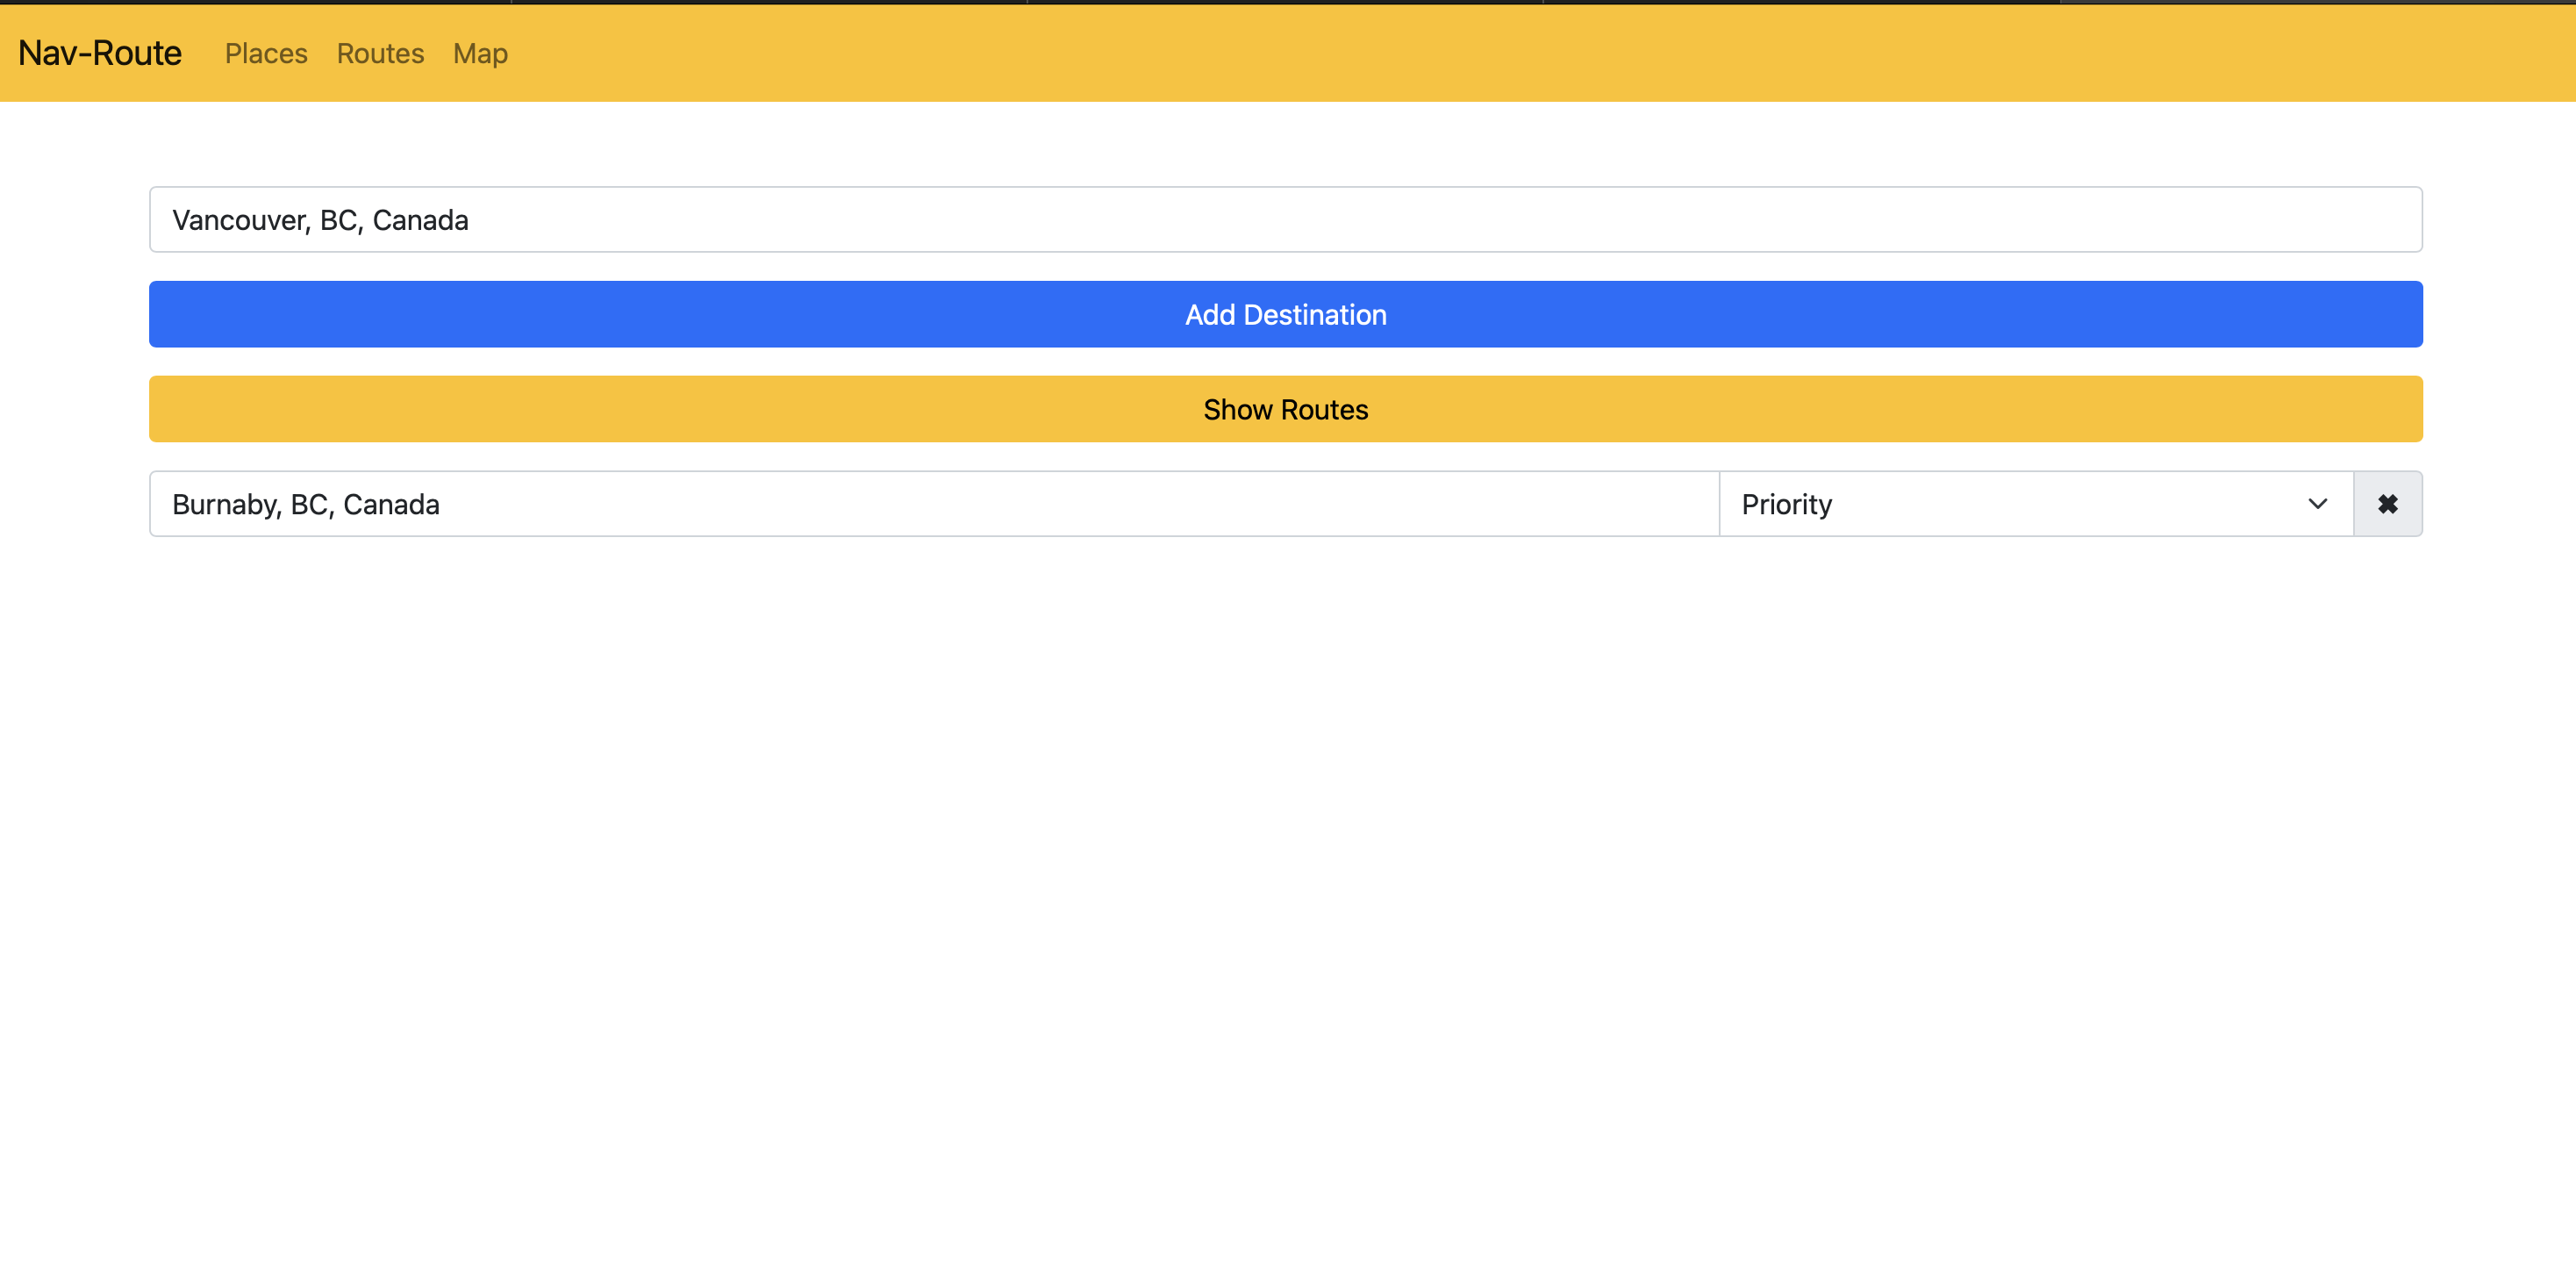
\includegraphics[width=1\textwidth]{NithishFinal/ARSS1.png}
  \caption{Alternative Route for Single Destination}
  \label{fig:example}
\end{figure}

\begin{figure}
  \centering
  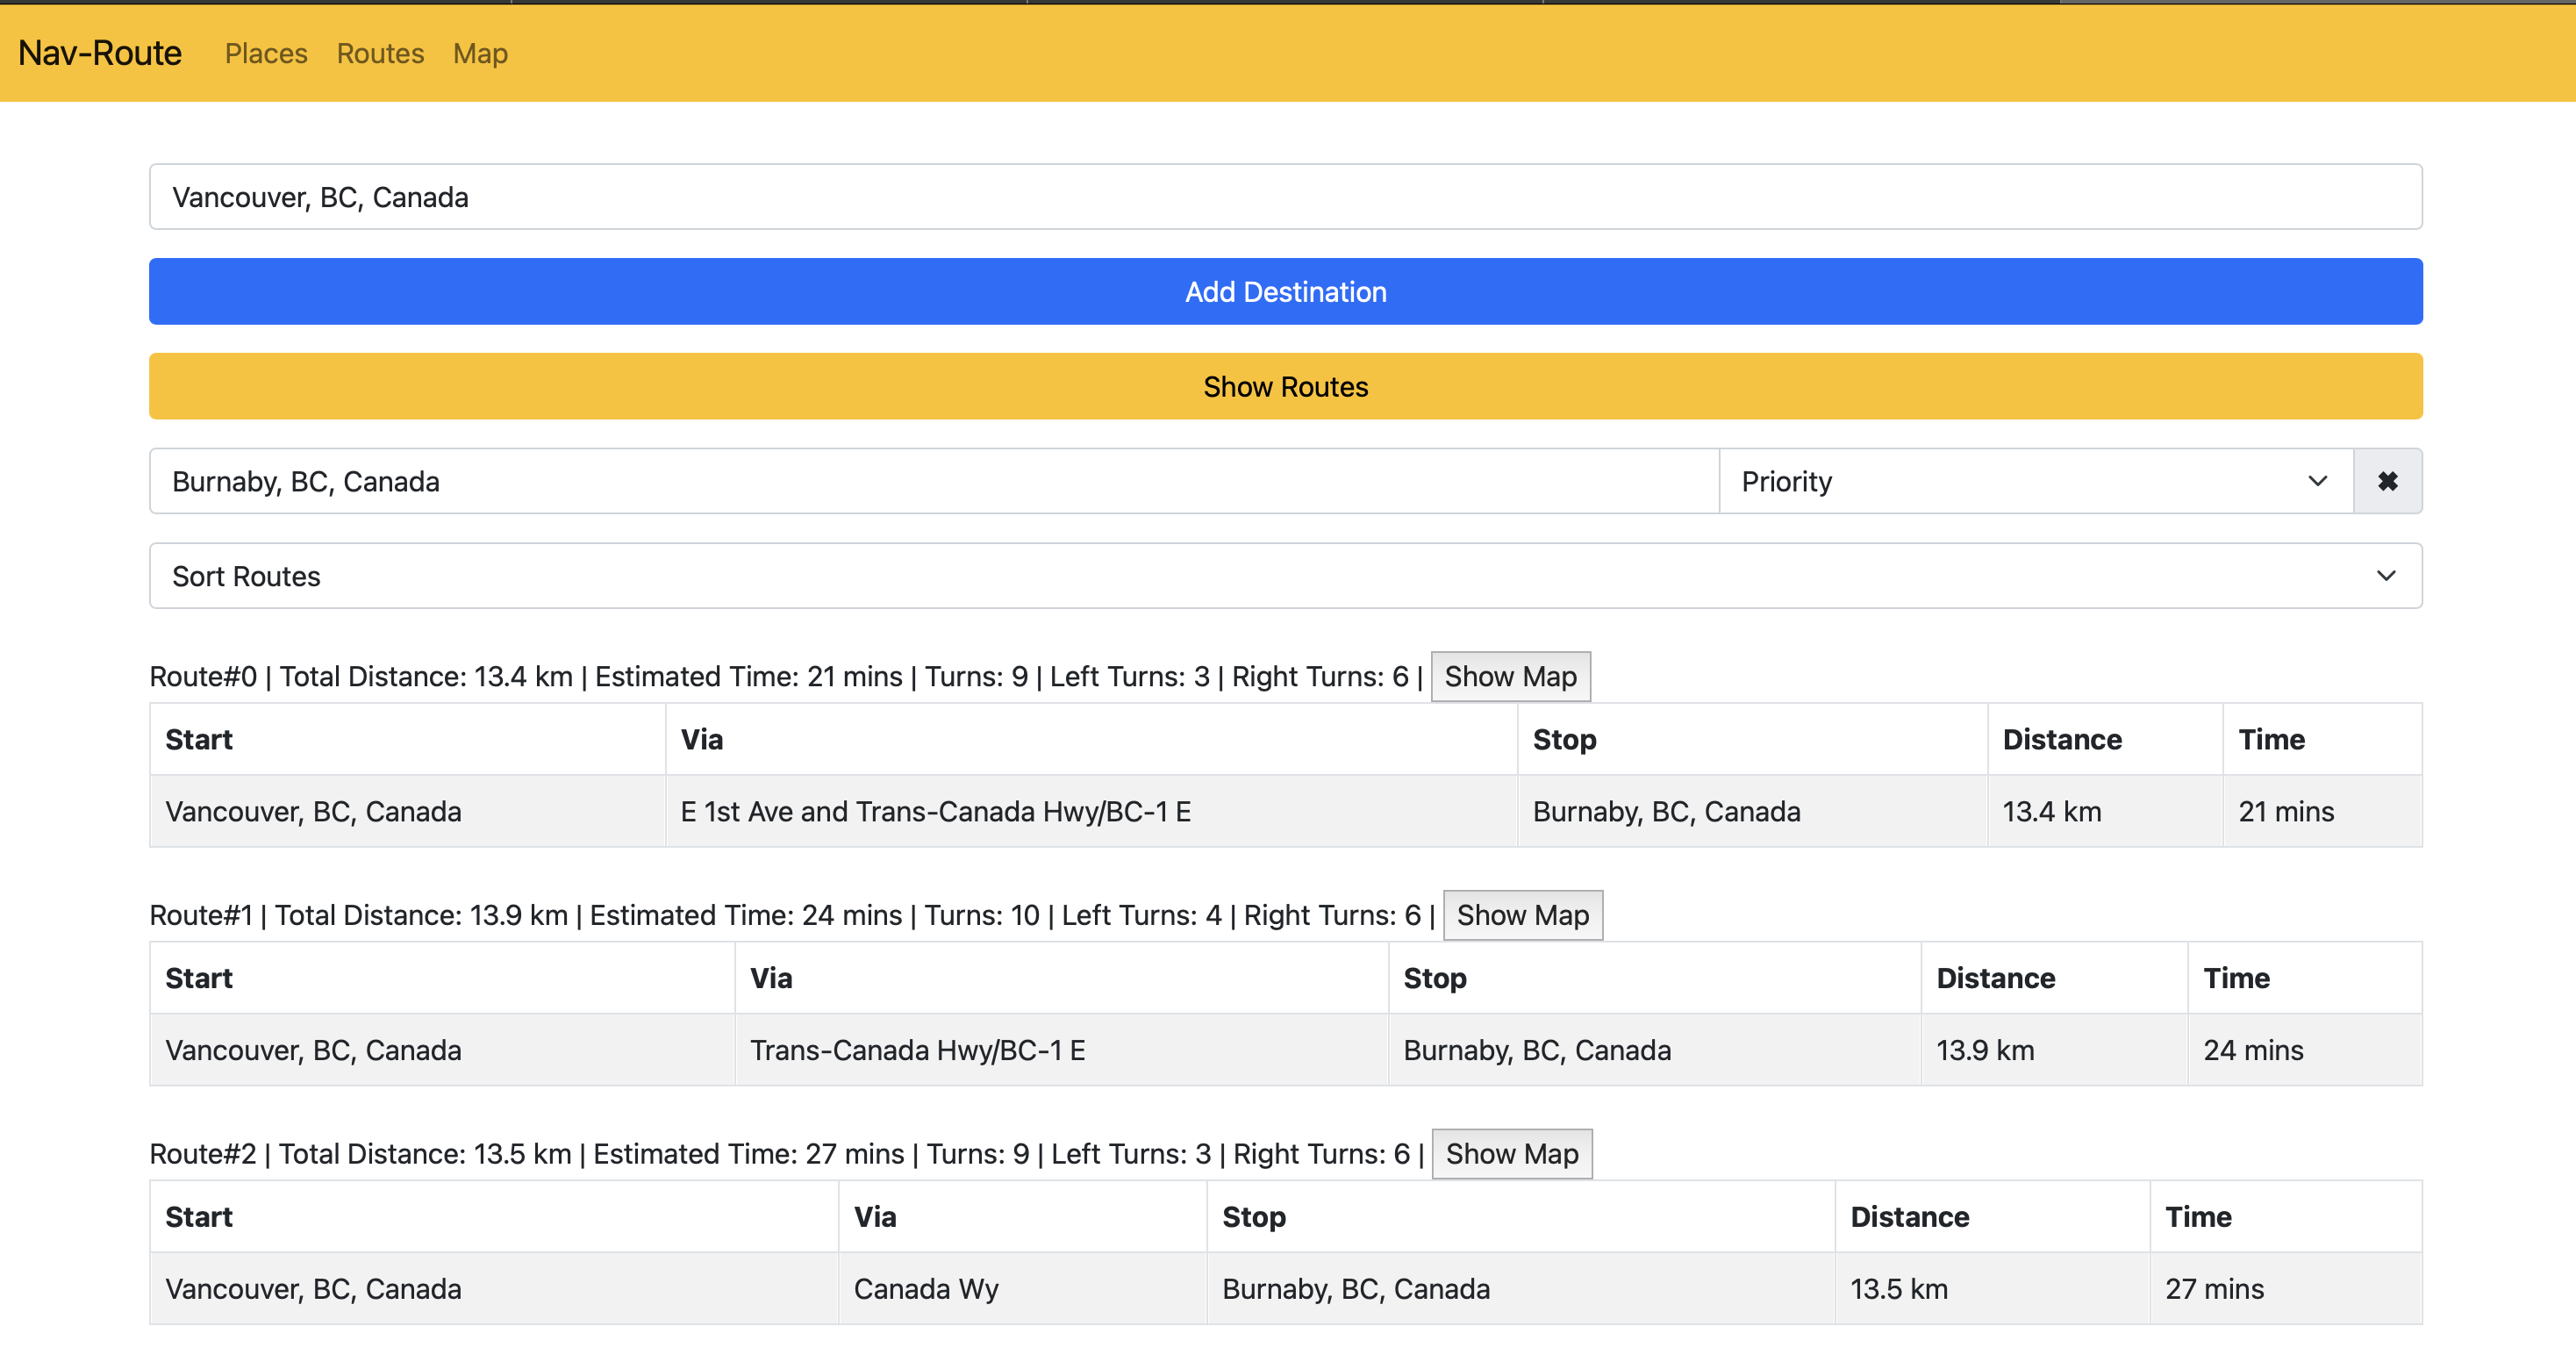
\includegraphics[width=1\textwidth]{NithishFinal/ARSS2.png}
  \caption{Multiple Routes}
  \label{fig:example}
\end{figure}

\begin{figure}
  \centering
  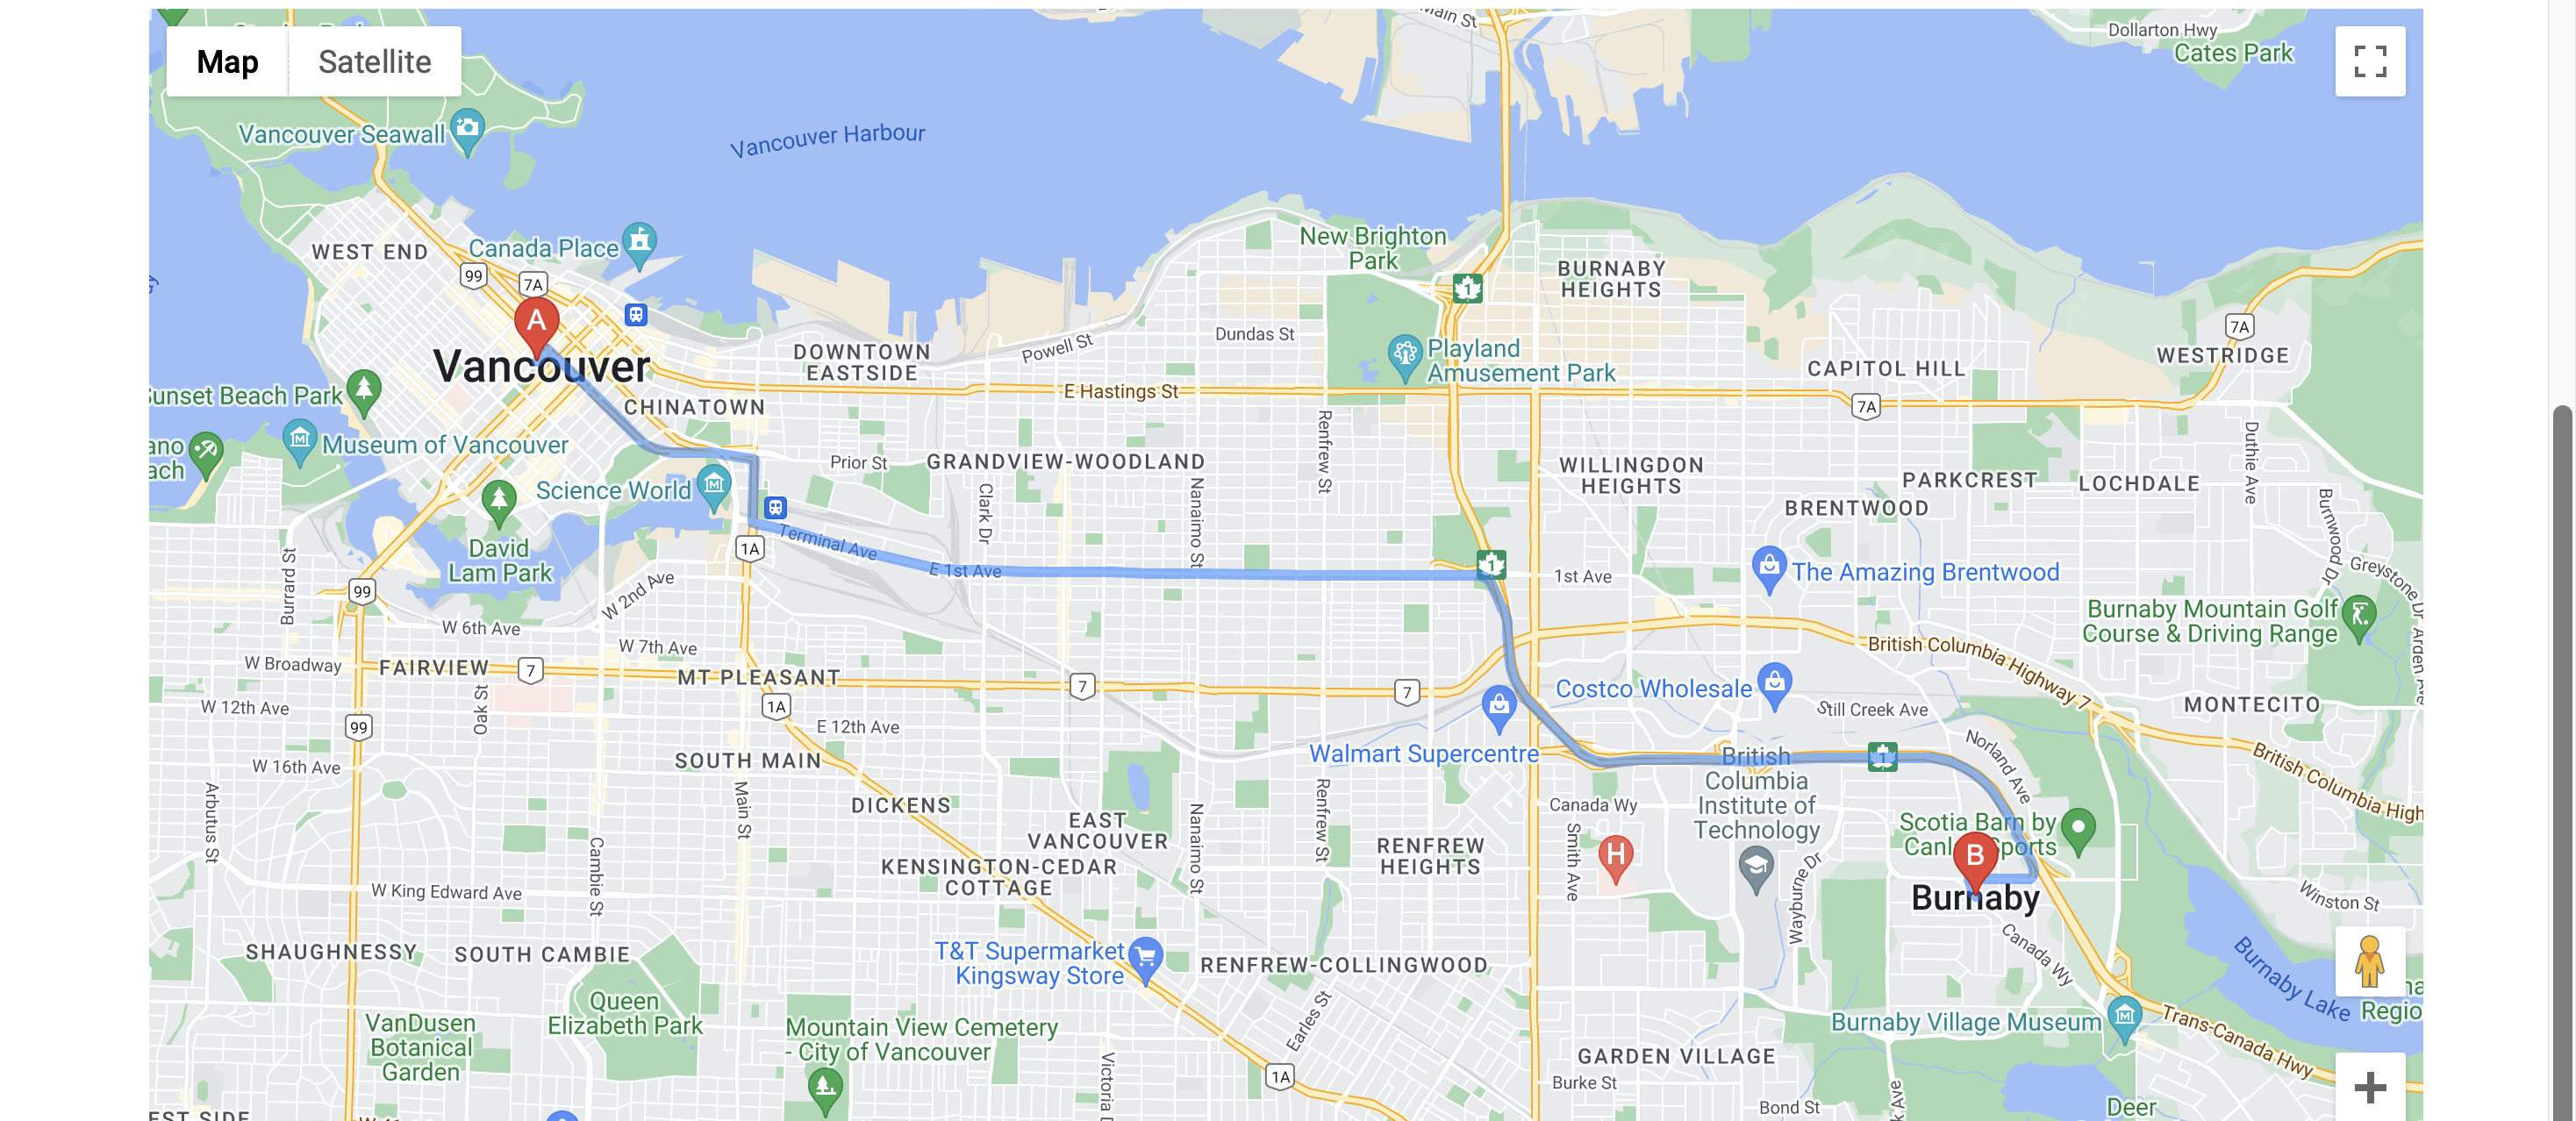
\includegraphics[width=1\textwidth]{NithishFinal/ARSS3.png}
  \caption{Display of Route on Map}
  \label{fig:example}
\end{figure}


\section{Conclusion}
As we approach the end of our capstone project, we are glad that we have been able to successfully implement and test the MVP and the project deliverable as proposed earlier. We attribute our success to the guidance we received from our professor under whose advice and direction and including the comprehensive planning, dedicated teamwork, and problem-solving approaches our team have shown, have enabled us to successfully complete our objectives.

\bibliography{FinalReport/FinalReport}

\end{document}
